\section{The binary--mixture confined between two walls}
The first system studied consisted of a binary--mixture of two fluids confined between two walls.
The fluid was prepared from a face--centered cubic lattice of spacing $1.64414 \sigma$ under a pressure of $P^{*} = 0.1$ and temperatures of $T^{*} = 0.8$ and $T^{*} = 0.9$, rnsuring the system exists withing the liquid region of the Lennard--Jones phase--space.\cite{Smit}
The pressure was controlled by applying an external force on one of the confining walls, which were bonded using a harmonic interaction to create a harmonic lattice.

\subsection{Using the Virial stress}
Initially the two systems were equilibrated for $2 \times 10^{6}$ timesteps (of length $\delta t = 0.001\ \tau$) which was sufficient to create the uniform number density consistent with a fluid state.
The simulations were then run for a further $40 \times 10^{6}$ timesteps over which period the number--density and Virial stress--tensor were spatially averaged into 400 spatial binds and outputted every timestep.
These values were then time-averaged using a block--length of $10 \tau$ in accordance with the results of the blocking--analysis described in Section 3.5 to produce profiles for the number--density and $\sigma_{xx}(z^{*})$ at $T^{*} = 0.8$ and $T^{*} = 0.9$, as shown in Figures \ref{PisVirRho} and \ref{PisVirStress}. 
Since the size of the box in the z--direction ($L_{z^{*}}$) varies for different temperatures when the pressure is held constant, the spatial averaging was done using a scaled coordinate $z'$ which corresponds to $z^{*} / L_{z^{*}}$.

\FloatBarrier
\begin{figure*}[h]
\centering
\includegraphics[scale=0.8]{PisVirRho}
\caption{PisVirRho caption goes here.}
\label{PisVirRho}
\end{figure*}

\begin{figure*}[h]
\centering
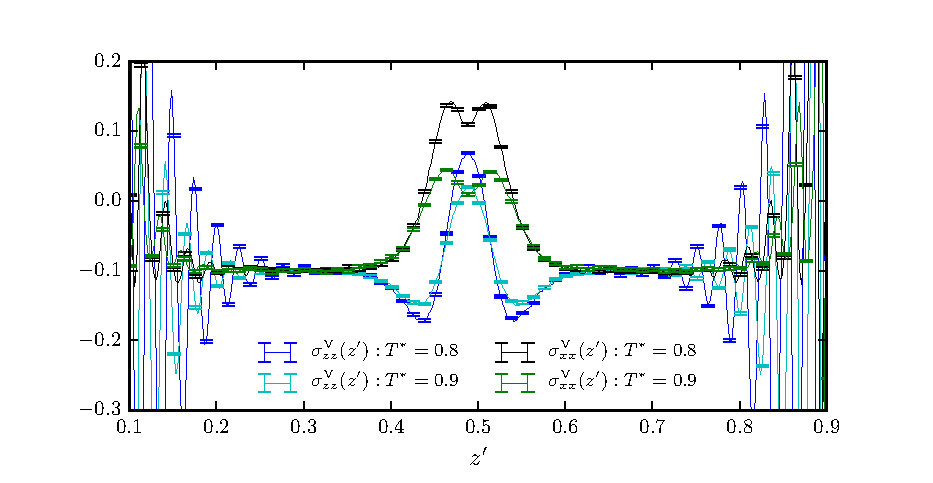
\includegraphics[scale=0.8]{PisVirStress}
\caption{PisVirStress caption goes here.}
\label{PisVirStress}
\end{figure*}
%COMMENT ON VIRIAL STRESS PROFILE AND NUMBER DENSITY

\FloatBarrier
The time--averaged values for the stress--tensor were then used to estimate the gradient of the stress--tensor with respect to temperature using Equation \ref{FinDiff}, shown in Figure \ref{PisVirForce}.
This gradient shows a clear peak at the interface of the two fluids, corresponding to the expected Marangoni force.
Importantly the force in the bulk of the fluid (far from both the interface and the walls) is zero within statistical error, which agrees with the prediction that there can be no force acting in a bulk fluid as the result of a temperature gradient.
In addition to this, there is also an oscillating force occuring at the surface of the wall which can be interpreted as a thermocapillary force (which notably could also be investigated using this method).
Since we are only interested in simulating the Marangoni effect, these thermocapillary forces were ignored and the central $1/3$ of the force profile was used to create an artifical Marangoni force using a temperature gradient of $\partial T^{*} / \partial x^{*} = 0.001$ and Equation \ref{ForceStressTemp}.

\begin{figure*}[h]
\centering
\includegraphics[scale=0.8]{PisVirForce}
\caption{PisVirForce caption goes here.}
\label{PisVirForce}
\end{figure*}
\FloatBarrier

This artfical body force was applied to an identical system prepared in the same way as before at $T^{*} = 0.85$.
A non-equilibrium simulation was run for $40 \times 10^{6}$ and x--component of the fluid velocity, $v^{*}_{x}$, was spatially and temporally averaged using the same blocking analysis 
This force profile was then applied as a body force to an identical system prepared at $T^{*} = 0.85$ and the x--component of the velocity was spatially and temporally averaged in an analogous way to the number--density and stress--tensor over $40 \times 10^{6}$ timesteps.
During this simulation the momentum of the walls in the $x$ and $y$ directions was fixed such that they provided a stationary reference point for the fluid.
As a result, the fluid shows a non-slip boundary condition at the walls and thus the walls act to hold the fluid far away from the interface at rest. 

\begin{figure*}[h]
\centering
\includegraphics[scale=0.8]{PisVirFlow}
\caption{PisVirFlow caption goes here.}
\label{PisVirFlow}
\end{figure*}
\FloatBarrier
The flow profile calculated for the fluid in this system is shown in Figure \ref{PisVirFlow}. 
This profile shows a sharp negative peak at the interface of the two fluids, indicating a Marangoni flow in the opposite direction to the temperature gradient as expected.
Furthermore the flow decay away from the interface is essentially linear which is consistent with a Couette flow arising from shear--driven fluid motion.








\subsection{The Finite Difference Approach}
Eqn. \ref{ForceStressTemp} shows that the body force due to a temperature gradient can be inferred from the temperature variation of the stress--tensor. 
To first order, the temperature gradient of the stress--tensor can be calculated using a finite difference approach across a small temparature variation as
\begin{equation}
\label{FinDiff}
\left( \frac{\partial \sigma_{xx}(z,x)}{\partial T} \right) \approx \frac{\sigma_{xx}^{T_{2}}(z,x) - \sigma_{xx}^{T_{1}}(z,x)}{T_{2} - T_{1}}.
\end{equation}
Using this approximation it should, in principle, be possible to compute the Marangoni flow profile for an interface as follows:
\begin{enumerate}
	\item Compute $\sigma_{xx}(z)$ for an equilibrium system at a given temperature $T_{1}$.
	\item Repeat the calculation for another equilibrium system at slightly higher temperate $T_{2}$.
	\item Approximate the temperature gradient of the stress tensor using the finite difference approach (Eqn. \ref{FinDiff}).
	\item Infer $f_{x}(z)$ using Eqn. \ref{ForceStressTemp} to calculate a force profile.
	\item Compute the flow profile by applying $f_{x}(z)$ as an artifical body force to a non-equilibrium simulation at a suitable intermediate temperature $T_{3}$ (i.e. $T_{1} < T_{3} < T_{3}$).
\end{enumerate}

This method is used in the remainder of this chapter to investigate the Marangoni flow arising at a liquid--liquid interface. 

\subsection{Using a periodic binary-mixture}
The purest system to study is the case of a symmetrical binary--mixture under three-dimensional periodic boundary conditions, whereby the only deviation from a simple bulk fluid is the presence of two interfaces within the periodic unit box. 
In this case and forces arising within the fluid can only arise from the effects of the interfaces on the fluid.

This system can be generated using a Lennard--Jones fluid by controlling the relative interaction strengths of the two fluids (henceforth referred to as Fluid A and Fluid B).
To achieve a suitable level of miscibility of the fluids the values $\epsilon_{AA} = \epsilon_{BB} = 1.0$ and $\epsilon_{AB}=0.55$ were used, in agreement with the previous studies on symmetrical Lennard--Jones binary mixtures.\cite{MorenzoRazo,Blas}
The pressure was chosen to be $P=0.1$ and the temperature values used were $T=0.8$ and $T=0.9$, ensuring that for all simulations the system exists within the liquid region of the pLennard--Jones phase space.\cite{Smit}
With an absence of any bounding walls in the system, the fluid pressure and temperature were controlled using a Nos\'{e}--Hoover barostat and thermostat.

